\documentclass{beamer}
\usepackage[english]{babel}
\setbeamertemplate{navigation symbols}{}
\setbeamertemplate{frametitle}[default][center]
\setbeamertemplate{bibliography item}{\insertbiblabel}
\usefonttheme[onlymath]{serif}

\usepackage{graphicx}
\graphicspath{ {./images/} }
\usepackage{amsmath}
\usepackage{wrapfig}

\title{Research Presentation}
\subtitle{COMP230}
\author{1706966}

\begin{document}

\begin{frame}
	\maketitle
\end{frame}

\begin{frame}{Background}
	Depression is a common illness worldwide, with more than 300 million people affected. When long-lasting and with moderate or severe intensity depression may become a serious health condition. At its worst, depression can lead to suicide. Close to 800 000 people die due to suicide every year. Suicide is the second leading cause of death in 15-29 year-olds\cite{DepressionStats}.
\end{frame}

\begin{frame}{The Issue}
	During this preliminary research it has been confirmed that there are no guidelines specific to the video game industry in regards to how suicide and depression are handled in video games.\vspace{5mm} %5mm vertical space
	
	Popularised guidelines do exist for portraying suicide in the news\cite{world2017preventing}\cite{nepon2009media} and drama adaptations\cite{DramaGuidelines}. \vspace{5mm} %5mm vertical space
	
	The drama adaptation guidelines match best with a video game environment and could possibly be implemented as guidelines for video games. However due to the artistic style, interactivity and immersion of video games it might be best to form more specific industry guidelines.   
\end{frame}

\begin{frame}{Importance}
	\begin{wrapfigure}{L}{0.5\textwidth} %this figure will be at the right
		\centering
		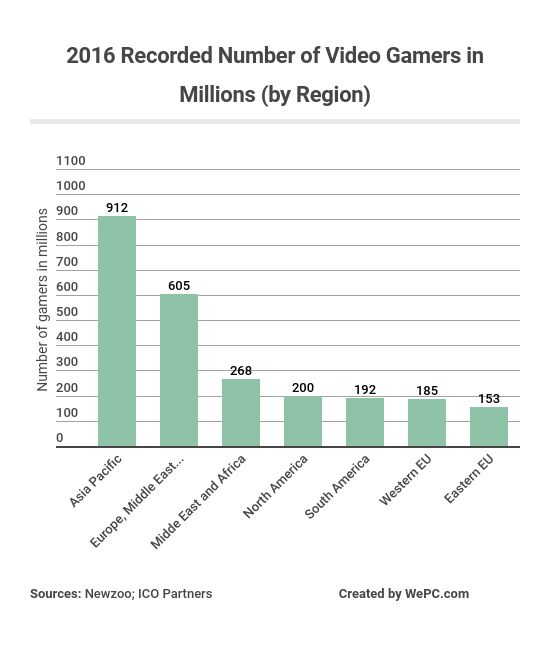
\includegraphics[width=0.5\textwidth]{numberOfGamers}
	\end{wrapfigure}
	With over 2.5 billion people playing video games the ability for games to deliver a message players is dramatic. Without general guidelines on how suicide and depression should be handled in video games its possible that they could be having a negative effect on the playerbase.
\end{frame}

\begin{frame}{National Statistics}
		\begin{itemize}
		\item 6,213 suicides in the UK and Ireland last year\cite{death2018suicide}.
		\item In the UK men are three times as likely to take their own lives than women, and in the Republic of Ireland four times as likely\cite{death2018suicide}.
		\item 19.7\% of over 16's in the UK showed symptoms of anxiety or depression in 2014\cite{MentalStatistics}.
		\item A higher proportion of women (22.5\%) than men (16.8\%) indicated they had some feelings of depression\cite{MentalStatistics}.
	\end{itemize}
\end{frame}

\begin{frame}{The Question}
	Should guidelines be put in place for video game developers to follow when portraying suicide/depression.
\end{frame}

\begin{frame}{Research Avenues}
	\begin{itemize}
		\item Would guidelines be seen as restrictive?
		\item Are current guidelines for media followed?
		\item Is there a positive outcome that comes from having guidelines?
	\end{itemize}
\end{frame}

\begin{frame}{Guidelines}
	Working together with charities that have experience in creating guidelines for the portrayal of suicide and depression in media\cite{world2017preventing}\cite{nepon2009media}. Also bringing in Take This\cite{TakeThis} a charity that helps provide support for those suffering with depression in the games industry to help make the guidelines specific to the industry.
\end{frame}

\begin{frame}{Too Restricting?}
	With games often being seen as an art form\cite{pearce2006games} there is a worry that developers will consider the guidelines to be restrictive. However as they are guidelines and not laws the presence of the guidelines will not stop developers from doing as they like, instead they will provide insight into good practice. Having the guidelines will at least urge the developers to think deeply about the consequences of the product they deliver.
\end{frame}

\begin{frame}{Outcome}
	Having guidelines widely available to the development community could help raise awareness about the issue of depression and aid in continuing to remove the stigma surrounding the discussion of mental illness. While effecting the community in this way the outcomes will trickle down into the gaming community itself as developers have more of an understanding about the issue.
\end{frame}

\begin{frame}{References}
	\bibliographystyle{ieeetran}
	\bibliography{references}
\end{frame}
\end{document}